%% PODSTAWOWE USTAWIENIA DOKUMENTU
\documentclass[12pt, a4paper, polish]{article}
%\usepackage[a4paper, lmargin=2.5cm, rmargin=2.5cm, hmargin=2.5cm, bmargin=2.5cm]{geometry}
\usepackage[a4paper,top=2cm,bottom=2cm,left=1cm,right=1cm]{geometry}
%\geometry{verbose,lmargin=2.5cm,rmargin=2.5cm}
\usepackage{enumerate}
% Symbole matematyczne
\usepackage{latexsym}
% Formatowanie czcionki
\usepackage[T1]{fontenc}
% Formatowanie polskich znaków
\usepackage{polski}
\usepackage[utf8]{inputenc}
% Akapit po sekcji
%\usepackage{indentfirst}
% Ustawienie nagłówków i stopek
\usepackage{fancyhdr}
% Liczba stron
%\usepackage{lastpage}
% Kolumny
%\usepackage{paracol}
% Czcionka latin modern
\usepackage{lmodern}
% Równania matematyczne
\usepackage{amsmath}
\usepackage{amsfonts}
\usepackage{amssymb}
\usepackage{amsthm}
% Wstawianie grafik
\usepackage{graphicx}
\usepackage[section]{placeins} % Ogarnięcie obrazków
\usepackage{float}
\usepackage{subcaption}
%\usepackage[outdir=./]{epstopdf}
\usepackage{grffile}
\usepackage{gensymb}

%% ODSTĘPY W WIERSZACH
\setlength{\parindent}{0.3cm}
\setlength{\parskip}{0.01cm}
\linespread{1}

%% SZARE TŁO TEKSTU
%\usepackage[most]{tcolorbox}
%\tcbset{
%	frame code={}
%	center title,
%	left=0pt,
%	right=0pt,
%	top=0pt,
%	bottom=0pt,
%	colback=gray!30,
%	colframe=white,
%	width=\dimexpr\textwidth\relax,
%	enlarge left by=0mm,
%	boxsep=5pt,
%	arc=0pt,outer arc=0pt,
%}

% HIPERŁĄCZA SPISU TREŚCI
\usepackage{hyperref}
\hypersetup{
	colorlinks,
	citecolor=black,
	filecolor=black,
	linkcolor=black,
	urlcolor=black
}

\begin{document}
	\fancyhf{}	% Usunięcie domyślnego stylu numerowania
	
	% ********************** TYTUŁ ****************************
	\noindent\textsf{\begin{Large}Laboratorium Sterowania Robotów Mobilnych\\\end{Large}
		Raport z zajęć\\
		Szymon Kacperek, Tomasz Smaruj \\
		AiR, studia stacjonarne II stopnia,  specjalność SSiR, rok akademicki 2020/2021\\
		\rule{\columnwidth}{0.2pt}}
	
	\thispagestyle{empty}
	\pagestyle{fancy}
	\fancyhead{}
	\rhead{\thepage}
	\renewcommand{\headrulewidth}{0pt}%{}
	\setlength{\footskip}{1mm}
	
	%							*****************POCZĄTEK DOKUMENTU*****************
	\tableofcontents
\section{Wstęp}

\section{Krótkie omówienie poszczególnych zadań sterowania i metod sterowania}
\subsection{Sterowniki wynikające z technik linearyzacji}
\subsection{Ciągły stabilizator Pometa jawnie zależny od czasu}
\subsection{Sterowniki nieciągłe metody VFO}

\newpage\section{Prezentacja wyników}
\subsection{Sterowniki wynikające z technik linearyzacji}
\subsubsection{Algorytm dla zadania odtwarzania pozycji}
\begin{figure}[H]
	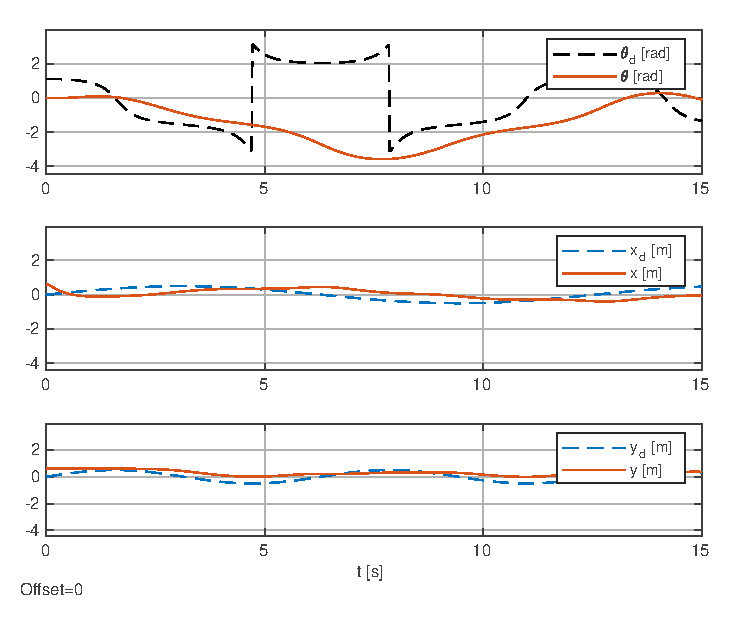
\includegraphics[width=0.5\linewidth]{lin/feedback/q.eps}
	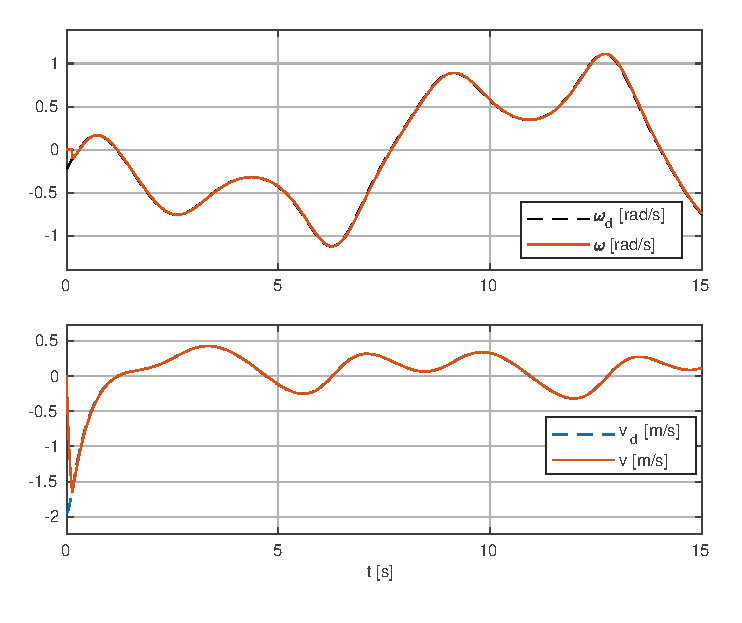
\includegraphics[width=0.5\linewidth]{lin/feedback/u.eps}\\
	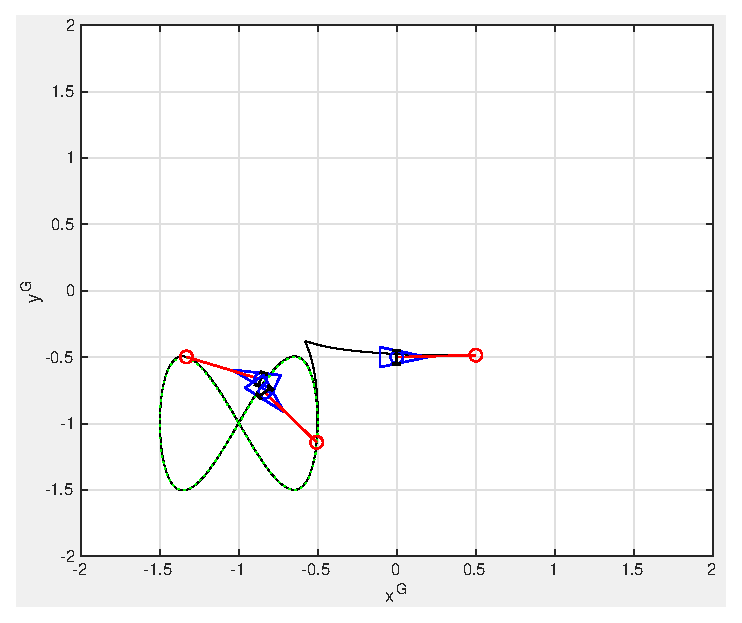
\includegraphics[width=0.5\linewidth]{lin/feedback/cartplot.eps}	
	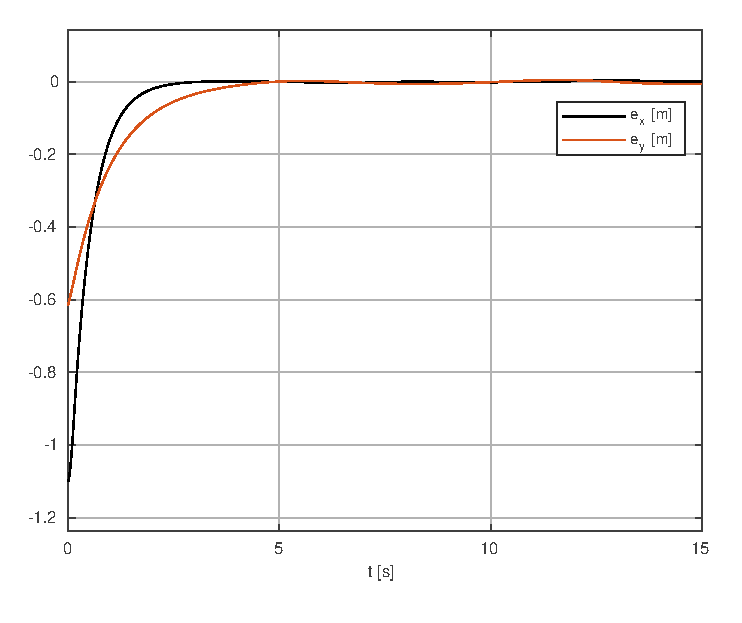
\includegraphics[width=0.5\linewidth]{lin/feedback/e.eps}	
\caption{Wyniki symulacji dla $L_Z=0.5[m]$ oraz $\beta_Z=0.3[\degree]$. Dobrano macierz wzmocnień $K$=\texttt{diag}$(2.0; 1.0)$. }\end{figure}


\begin{figure}[H]
	\subsubsection{Algorytm dla zadania śledzenia trajektorii}
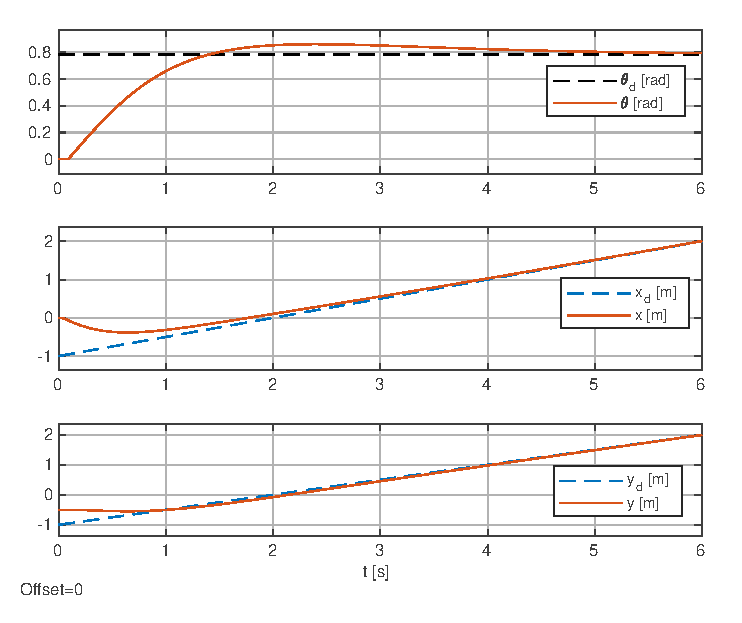
\includegraphics[width=0.5\linewidth]{lin/approx/q_tt.eps}
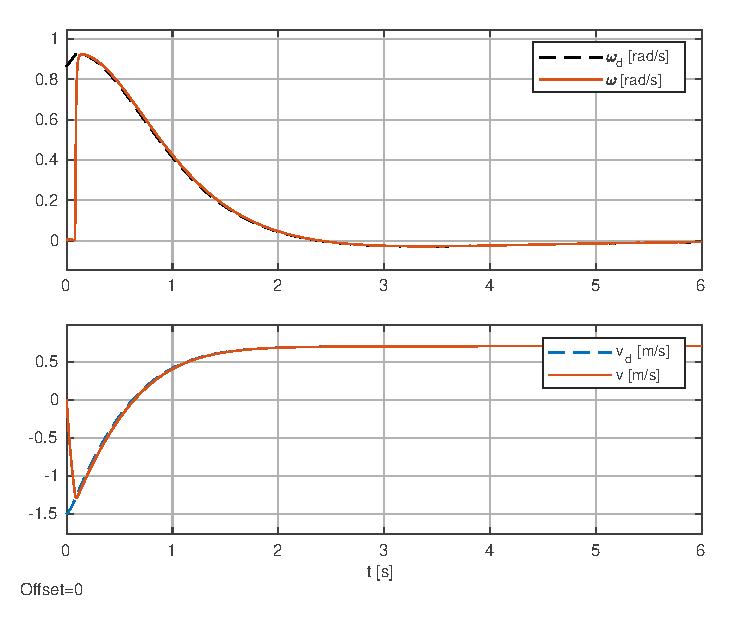
\includegraphics[width=0.5\linewidth]{lin/approx/u_tt.eps}\\
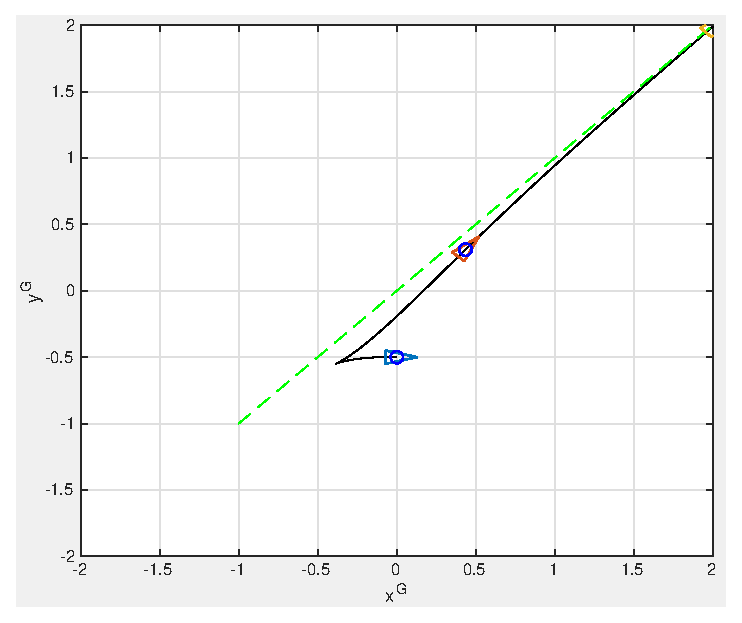
\includegraphics[width=0.5\linewidth]{lin/approx/cartplot_tt}	
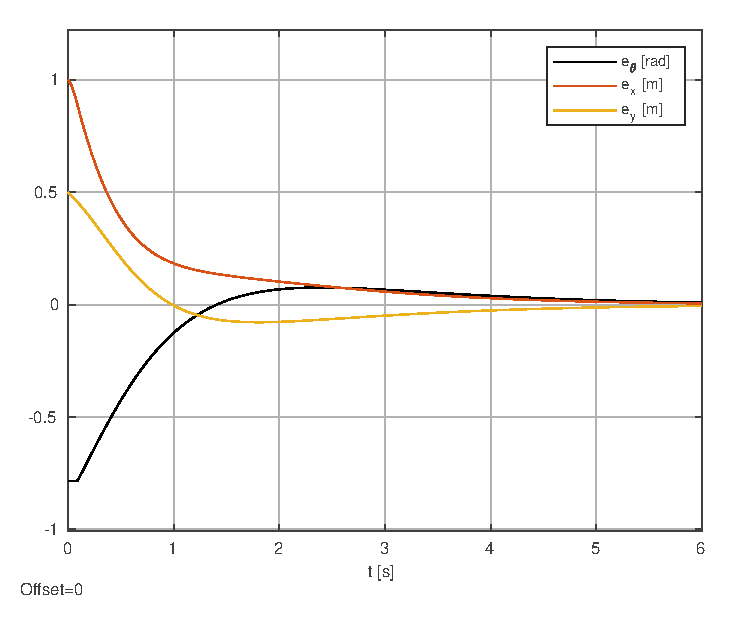
\includegraphics[width=0.5\linewidth]{lin/approx/e_tt.eps}
\caption{Wyniki symulacji dla współczynników $\zeta=1, \quad \alpha=2, \quad k_{22} = k_{11} = -2\zeta\sqrt{u_{d1}^2+\alpha u_{d2}^2}$ oraz $k_{13}=-\alpha u_{d2}$.}\end{figure}


\begin{figure}[H]
	\subsubsection{Algorytm dla zadania odtwarzania ścieżki}
	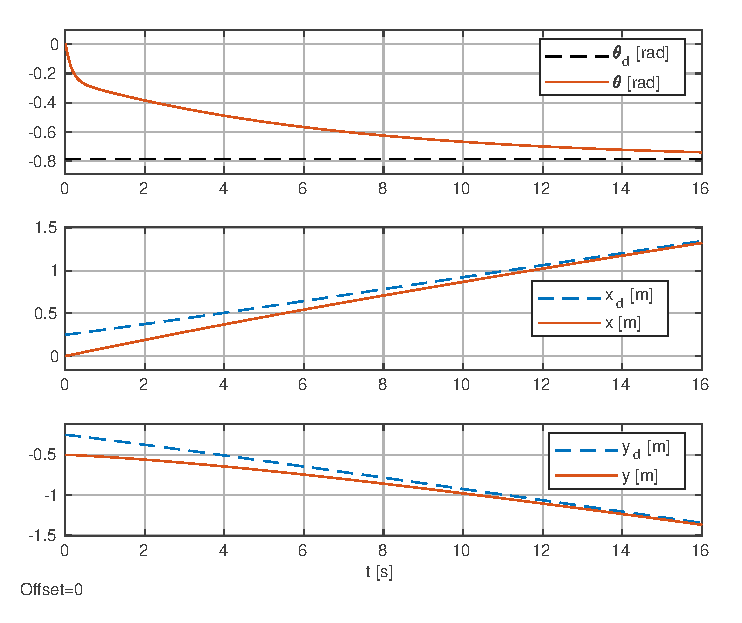
\includegraphics[width=0.5\linewidth]{lin/approx/q_pf.eps}
	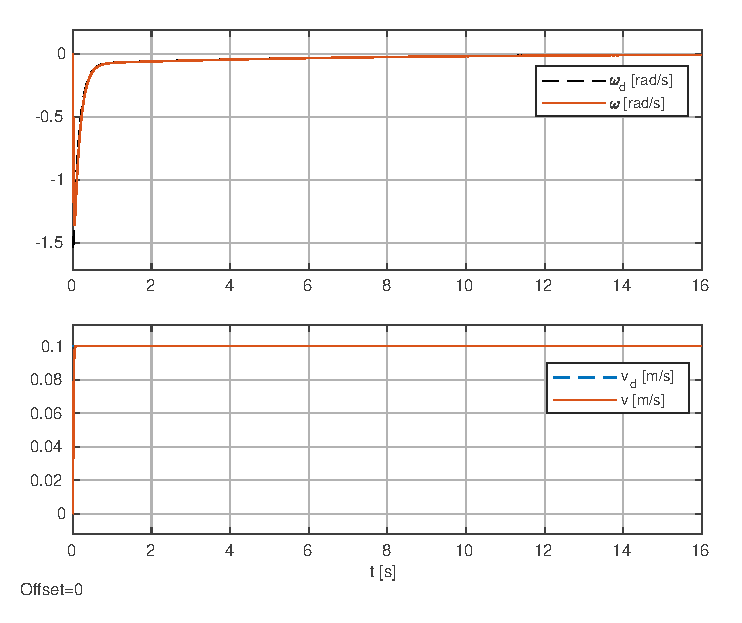
\includegraphics[width=0.5\linewidth]{lin/approx/u_pf.eps}\\
	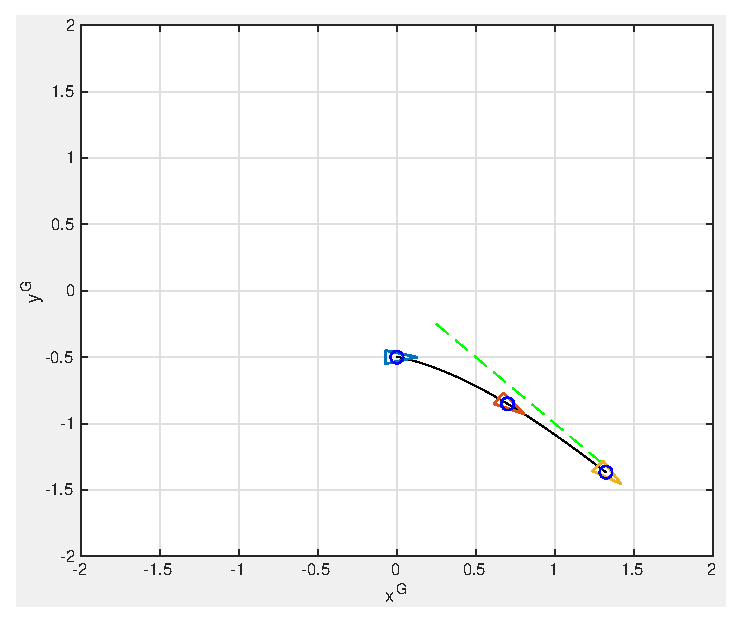
\includegraphics[width=0.5\linewidth]{lin/approx/cartplot_pf}	
	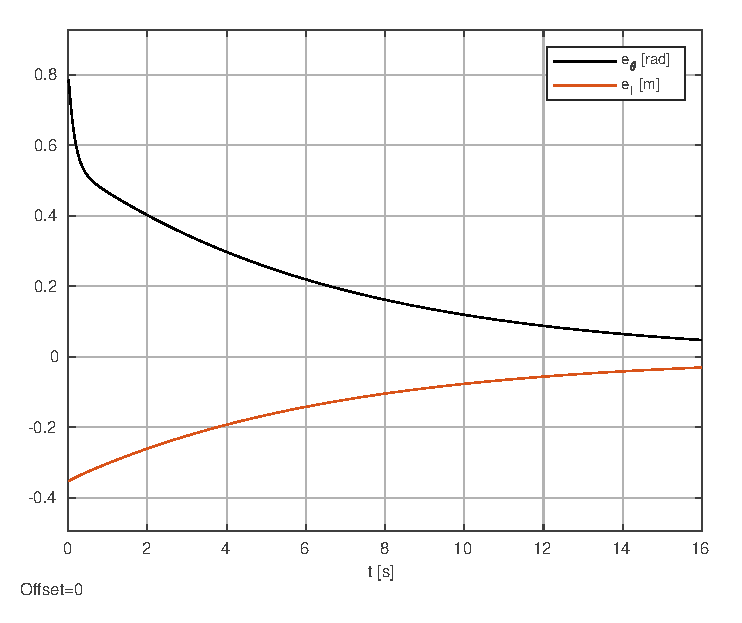
\includegraphics[width=0.5\linewidth]{lin/approx/e_pf.eps}
	\caption{Wyniki symulacji dla współczynników $\zeta=1, \quad \omega_n=3, \quad k_1 = 9, \quad k_2 = 6$.}\end{figure}


\begin{figure}[H]
\subsection{Ciągły stabilizator Pometa jawnie zależny od czasu}
	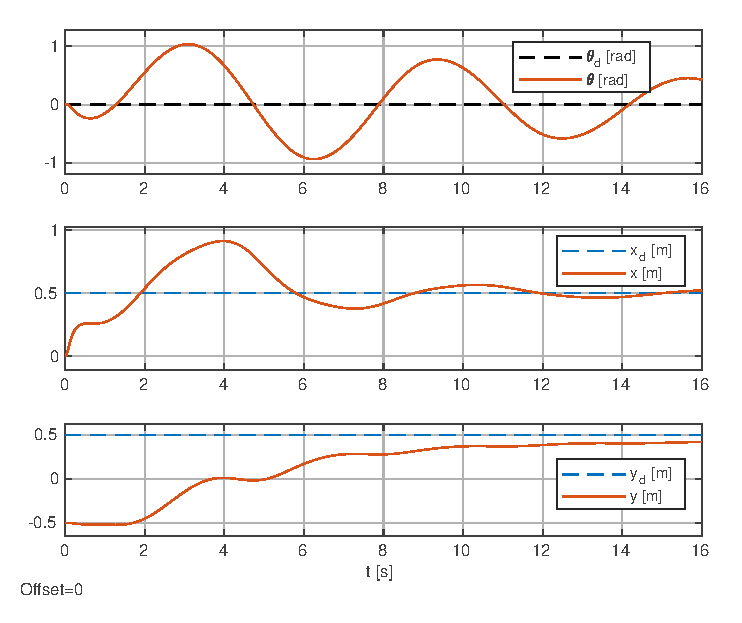
\includegraphics[width=0.5\linewidth]{pomet/q.eps}
	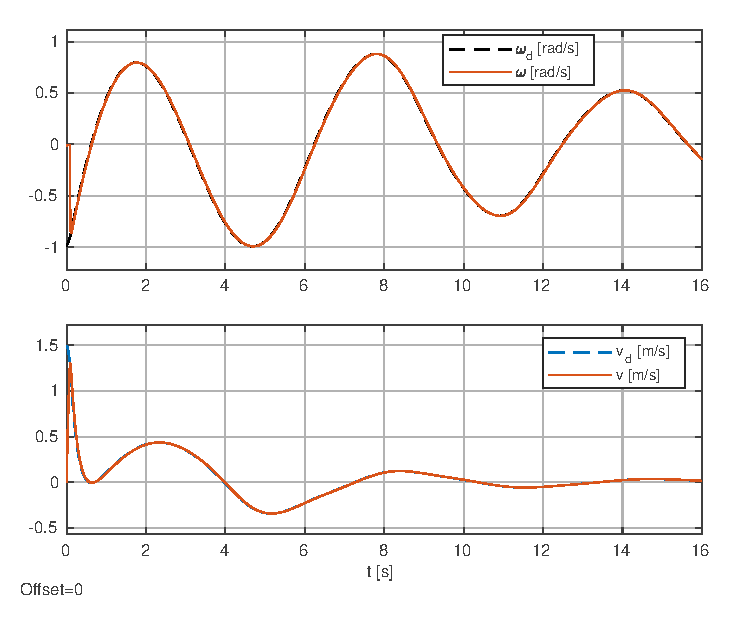
\includegraphics[width=0.5\linewidth]{pomet/u.eps}\\
	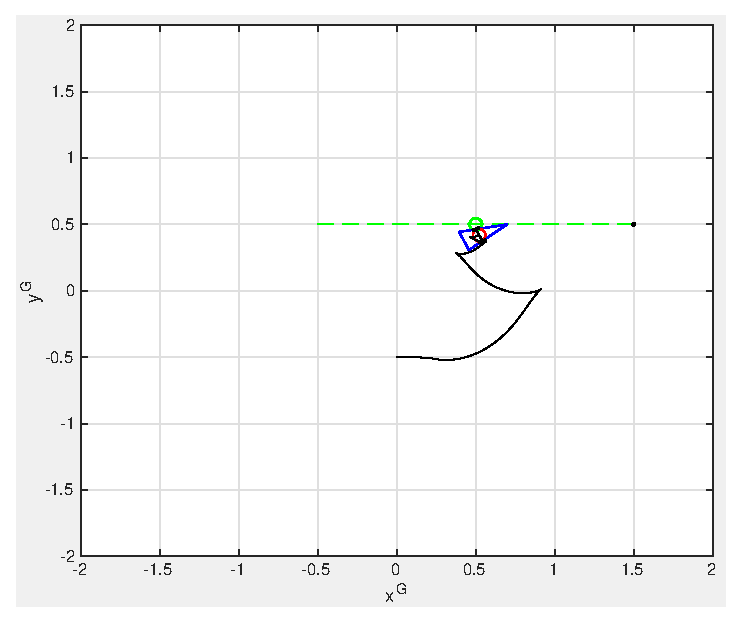
\includegraphics[width=0.5\linewidth]{pomet/cartplot.eps}	
	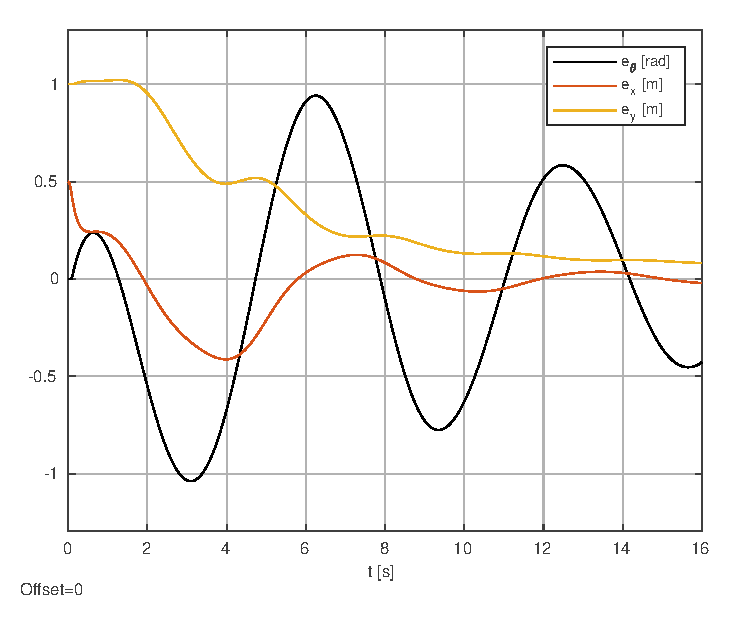
\includegraphics[width=0.5\linewidth]{pomet/e.eps}
	\caption{Wyniki symulacji dla przyjętych współczynników $k_1=k_2=k_3=k_4=1, \quad \delta_p=0.01, \quad \Omega=1$.}\end{figure}
\subsection{Sterowniki nieciągłe metody VFO}

\begin{figure}[H]
\subsubsection{Algorytm VFO dla zadania śledzenia trajektorii}
	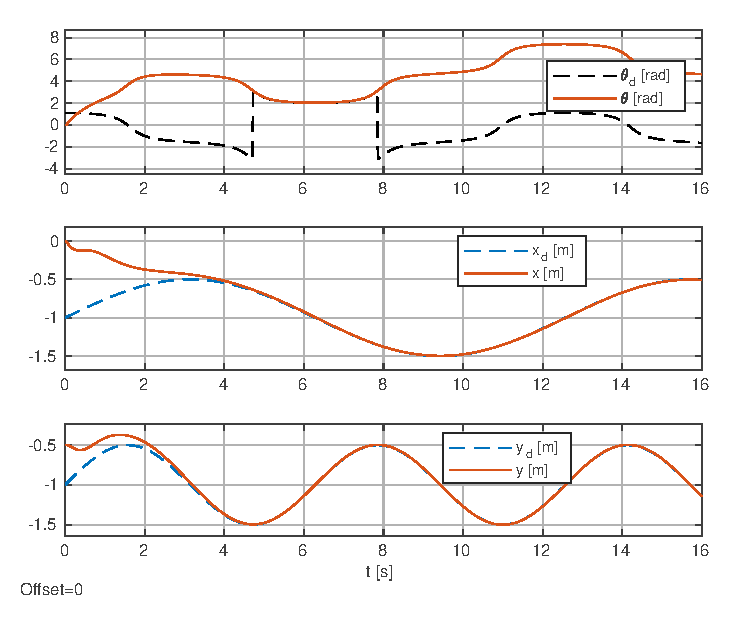
\includegraphics[width=0.5\linewidth]{vfo/q_tt.eps}
	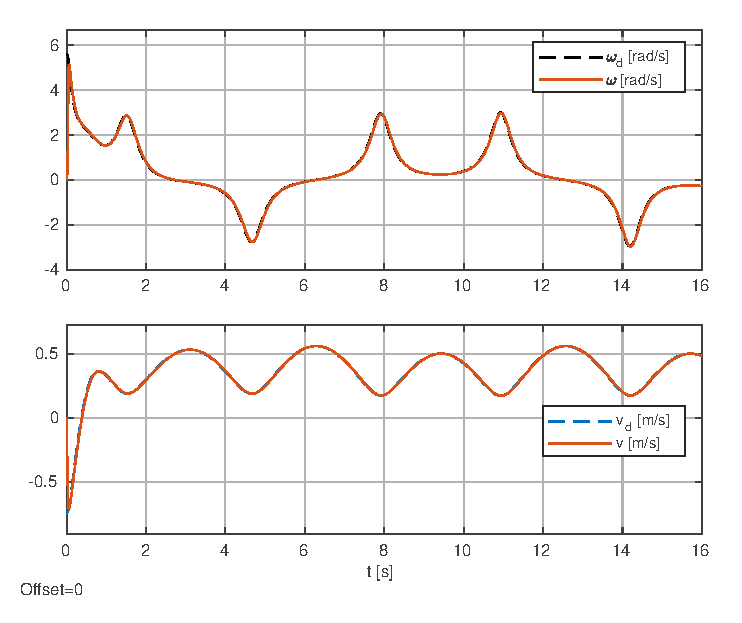
\includegraphics[width=0.5\linewidth]{vfo/u_tt.eps}\\
	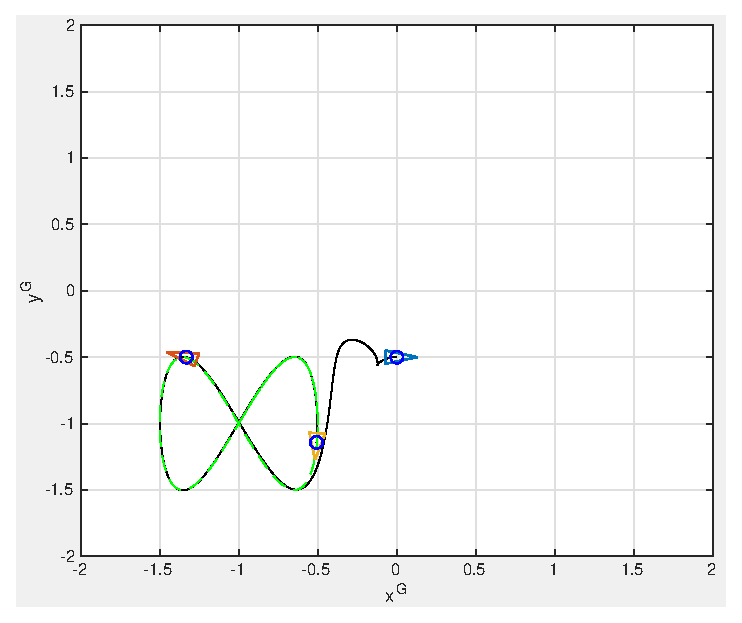
\includegraphics[width=0.5\linewidth]{vfo/cartplot_tt.eps}	
	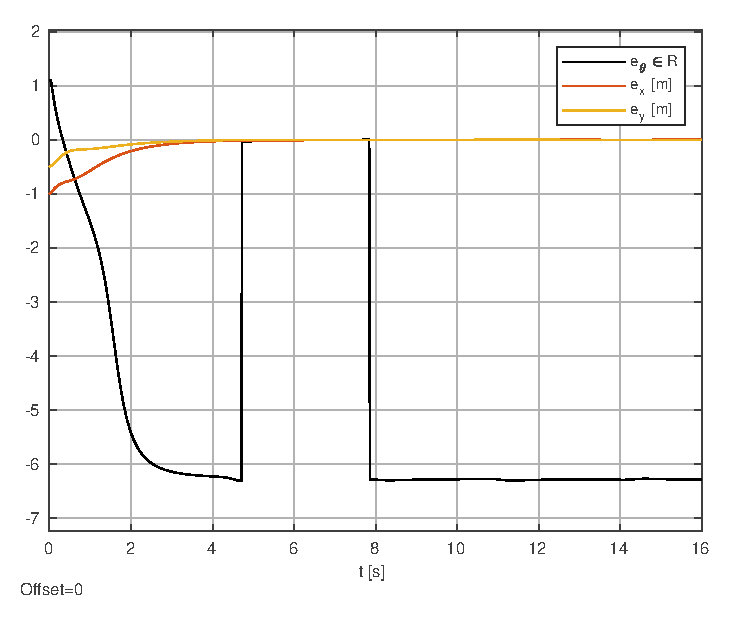
\includegraphics[width=0.5\linewidth]{vfo/e_tt.eps}
	\caption{Wyniki symulacji dla przyjętych współczynników $\zeta_d=1,\quad k_p =1, \quad \eta=0.8k_p,\quad \delta=0.001,\quad k_a=2k_p$.}\end{figure}

\begin{figure}[H]
	\subsubsection{Algorytm VFO dla zadania podążania do punktu}
	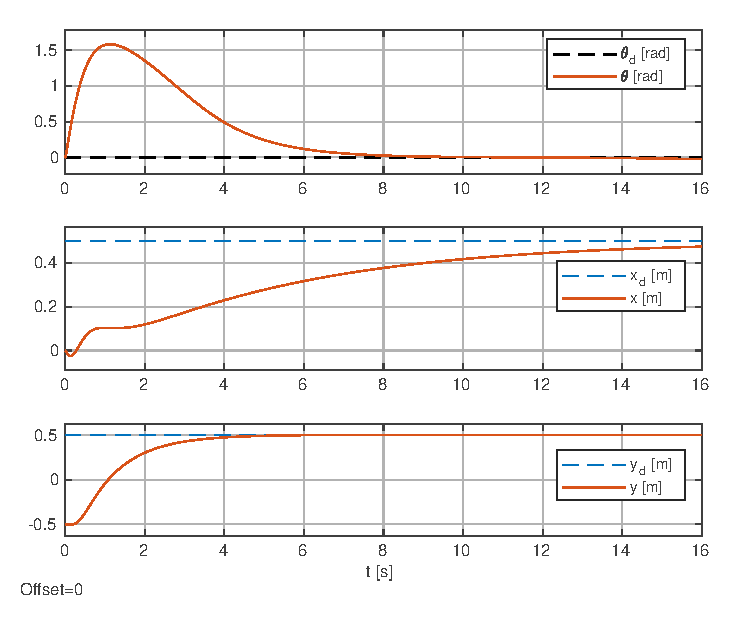
\includegraphics[width=0.5\linewidth]{vfo/q_ps.eps}
	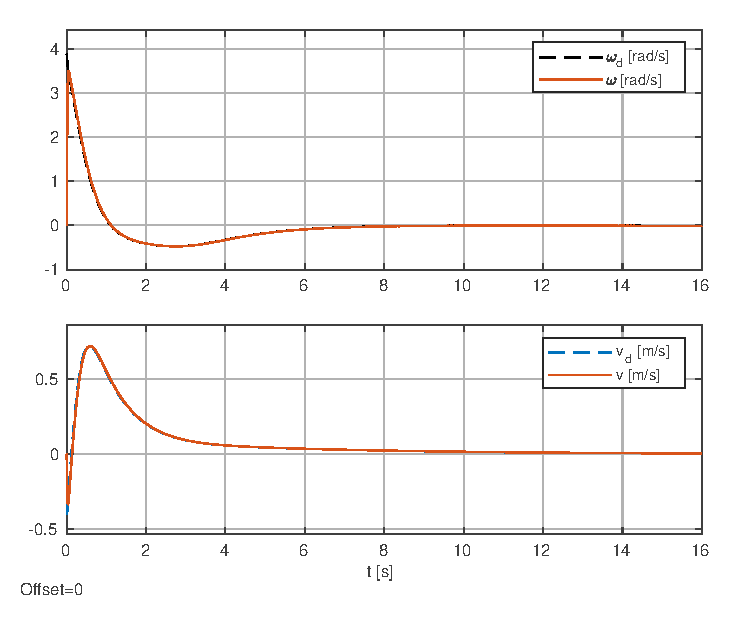
\includegraphics[width=0.5\linewidth]{vfo/u_ps.eps}\\
	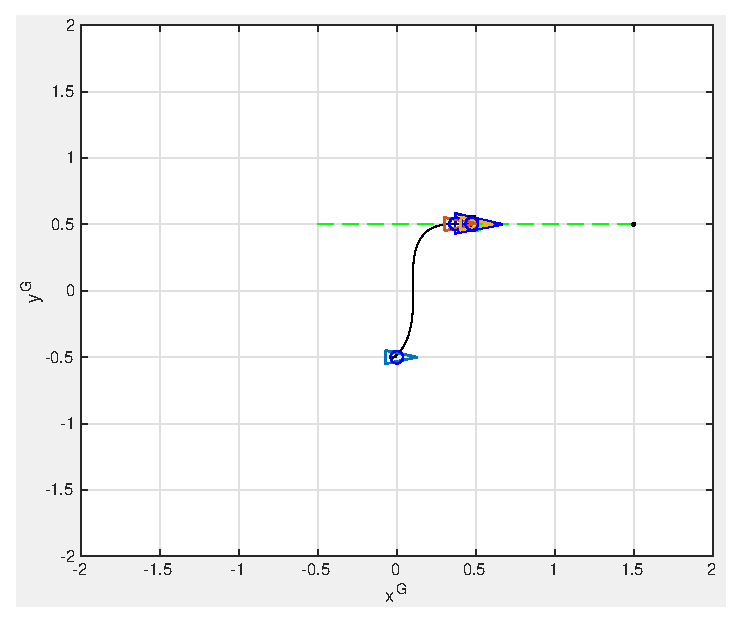
\includegraphics[width=0.5\linewidth]{vfo/cartplot_ps.eps}	
	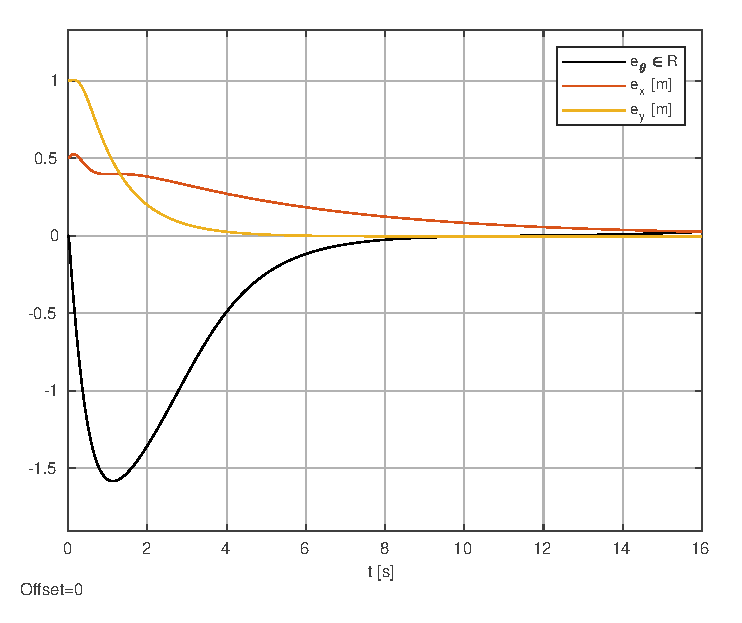
\includegraphics[width=0.5\linewidth]{vfo/e_ps.eps}
	\caption{Wyniki symulacji dla przyjętych współczynników $\zeta_d=1,\quad k_p =1, \quad \eta=0.8k_p,\quad \delta=0.001,\quad k_a=2k_p$.}\end{figure}


\newpage\section{Analiza wyników}
\section{Wnioski}


\end{document}
